% =====================================================================
% Paper 4 - "What the Variant Tables Erased"
% COMPILE WITH: XeLaTeX  (not pdfLaTeX) -- needed for Chinese characters.
% Self-contained: uses only TeX Live / Overleaf bundled packages and fonts
% (ctex pulls the bundled Fandol CJK font, so no font-not-found errors).
% Two-column ACL-style layout. Plain hyphens only.
% Figure: upload fig_results.png (from results/) to the same Overleaf project.
% =====================================================================
\documentclass[10pt,twocolumn]{article}

\usepackage[a4paper,top=2.0cm,bottom=2.3cm,left=1.9cm,right=1.9cm,columnsep=0.65cm]{geometry}
\usepackage[UTF8,scheme=plain]{ctex}   % Chinese support, auto bundled font (XeLaTeX)
\usepackage{amsmath,amssymb}
\usepackage{booktabs}
\usepackage{graphicx}
\usepackage{caption}
\usepackage{microtype}
\usepackage[hidelinks]{hyperref}

\captionsetup{font=small,labelfont=bf,skip=5pt}
\setlength{\parindent}{1em}
\setlength{\belowcaptionskip}{2pt}
\setlength{\textfloatsep}{10pt plus 2pt minus 2pt}

% Title is typeset manually inside \twocolumn[...] below (do NOT use \maketitle
% in a twocolumn class: it nests \twocolumn and errors).

\begin{document}
\twocolumn[{%
  \vspace*{0.2em}
  \begin{center}
    {\large\bfseries What the Variant Tables Erased: The 1955 First List of
    Processed Variant Characters, the Distinctions It Removed, and Their
    Survival in Taiwan and in Language Models\par}
    \vspace{0.7em}
    {\normalsize Aryan Maity\par}
    \vspace{0.2em}
    {\small St.~Edmund's College \quad\textbar\quad
     \texttt{github.com/aryan35790jp/cross\_straight\_chinese}\par}
  \end{center}
  \vspace{1.0em}
  \begin{center}
  \begin{minipage}{0.86\textwidth}
  \begin{center}\textbf{Abstract}\end{center}
  \small\noindent
When mainland China reformed its writing system it ran two separate reforms, not
one. The first, simplification, reduced and merged character shapes. The second,
variant abolition, is far less studied: the 1955 First List of Processed Variant
Characters declared 1,025 characters to be redundant variants of a chosen
orthodox form and removed them from print. Taiwan never adopted this list and
preserves the abolished forms as standard. We treat the 1955 table as a
measurable event. Building the complete population of 796 groups directly from
the official table and the Unicode Han database with no manual annotation, we
quantify what the abolition removed. As an upper bound, the collapse created
922.2 bits of written-form sense uncertainty, of which 90.9 percent is
unrecoverable from pronunciation, almost exactly the 92.3 percent we previously
measured for simplification. The grounded picture is sharper: roughly three
quarters of the abolition was genuine redundancy, while 204 groups (25.6 percent)
carried a documented distinction, concentrated in 71 reading-bearing groups and
in surname and place-name uses that the original 1955 notice itself acknowledged
it was sacrificing. We then probe five language models that share an identical
token vocabulary for our characters, and find a sharp double dissociation. The
representation of the abolished \emph{forms} depends strongly on script:
Traditional-trained models keep each abolished variant distinct from its orthodox
counterpart, while Simplified-trained models collapse it (Cliff's delta = 0.78 on
real variant tokens, $p \approx 10^{-89}$). Because the token vocabulary is held
identical across the panel, this is a property of the learned weights, not of
tokenization. The recovery of \emph{meaning} from context behaves oppositely: it
does not differ by script at all, but it is specific to genuine distinctions,
recovering the reading-level senses the abolition merged while leaving redundant
allographs unrecovered (Cliff's delta = 0.26, $p = 0.02$, calibrated against a
label-shuffle null). Form follows the script that preserved it; sense follows the
distinction that was real. As an external check, the abolished variants that the
state itself later restored prove to be distinction-bearing at more than twice the
base rate ($p < 0.001$): the annotation-free measure predicts the language
authority's own reversals. The Traditional orthography that Taiwan preserves is,
in a measurable sense, a record of distinctions the variant tables removed.
  \end{minipage}
  \end{center}
  \vspace{1.4em}
}]

\section{Introduction}
The standard account of the mainland Chinese script reform is a story about
stroke counts. A second, quieter reform ran alongside it. In December 1955 the
Ministry of Culture and the Chinese Character Reform Committee issued the First
List of Processed Variant Characters (第一批异体字整理表), which grouped
characters judged to be variants of one another, chose one form in each group as
orthodox, and abolished the rest. The original list contained 810 groups and
removed 1,055 characters; after later adjustments it stands at 796 groups. Taiwan
did not adopt the list. The abolished forms remain standard there and are
documented in full by the Ministry of Education variant dictionary.

The two reforms are usually conflated, but they are different events with
different mechanisms. Simplification reduced and merged shapes; we have elsewhere
measured the meaning it destroyed and shown that language models inherit the
collapse \cite{maity2025simplification}. Variant abolition is a deletion of
redundancy by decree, and the decisive empirical question is whether the deleted
forms were in fact redundant. The reform assumed they were. The historical record
suggests otherwise in part: the 1955 notice itself carved out an exception for
variants used as surnames, permitting them ``only for use as a surname,'' and the
state later restored characters such as 邱 and 於 after the merger broke names. No
one, to our knowledge, has quantified how much distinction the table removed, nor
asked whether language models carry a trace of it.

This paper does both. Our contributions are:
\begin{itemize}
\setlength{\itemsep}{1pt}
\item A complete, annotation-free reconstruction of the 1955 population (796
groups, 1,821 characters) from the official table and Unicode, with a
phonological and semantic typology of each group.
\item An information-theoretic account of what the abolition removed, including
the result that 90.9 percent of the upper-bound distinction is unrecoverable from
pronunciation, and the grounded finding that about a quarter of the abolition was
distinction-bearing rather than redundant.
\item A five-model, shared-vocabulary probe that reveals a double dissociation:
the representation of the abolished \emph{form} is sharply controlled by script
orientation (Cliff's delta $= 0.78$, a weight-level effect), while the recovery
of its \emph{sense} from context is script-independent but specific to genuine
distinctions.
\item An external validation: the abolished variants that the state itself later
restored are distinction-bearing at more than twice the base rate
($p < 0.001$), so the annotation-free measure predicts the language authority's
own policy reversals.
\end{itemize}

\section{Background and Related Work}
\noindent\textbf{Two reforms, not one.} The simplification of character shapes
(简化字) and the abolition of variants (异体字整理) were issued as separate
documents with separate rationales. Simplification is heavily studied; the
variant table is known mainly to specialists in the history of the reform, where
it is discussed qualitatively, often through the controversies it caused for
surnames and place names. We are not aware of prior work that quantifies the
distinction it removed or probes its trace in neural representations.

\noindent\textbf{Conversion is not our question.} Computational work on the two
scripts concentrates on conversion \cite{opencc}, where the hard direction is
Simplified to Traditional. Our question is orthogonal: not whether a system can
recover the right form, but how much distinction the abolition discarded and
whether a model trained on text that kept the forms represents them differently.

\noindent\textbf{Representational probing.} A large literature decodes lexical
and sense structure from contextual embeddings \cite{tenney2019,hewitt2019}. We
use the silhouette coefficient \cite{rousseeuw1987} under cosine distance to
measure how separable two senses are in a model's representation, and we
calibrate every separability measure against a per-group label-shuffle null,
keeping the statistical claims conservative.

\section{The 1955 Population and Its Typology}
\noindent\textbf{Construction.} We parse the complete adjusted table directly
from its official text and attach to every character its Mandarin reading,
English gloss, and Kangxi radical from the Unicode Han database \cite{unihan}. No
step uses manual annotation. The result is 796 groups covering 1,821 characters:
605 groups of two members, 158 of three, and 33 of four or more. The orthodox
form is the retained standard; the bracketed members are the abolished variants
(1,025 in total).

\noindent\textbf{Phonological typology.} Comparing the Mandarin reading of each
variant to its orthodox form, a group is \emph{heterophonic} if some variant
differs in segment (查 ch\'a vs 査 zh\=a, the surname), \emph{tonal-variant} if it
differs only in tone, and \emph{homophonic} otherwise.

\noindent\textbf{Semantic typology.} A group is \emph{distinct-gloss} if a
variant carries gloss content the orthodox form does not. We call a group
\emph{distinction-bearing} if it is reading-bearing (heterophonic or
tonal-variant) or distinct-gloss, and \emph{redundant-control} otherwise
(homophonic with no gloss difference: a presumed true allograph). This yields 204
distinction-bearing groups, 25.6 percent of the table (Table~\ref{tab:typology}).
To guard the gloss signal against the gloss language, we cross-check it against
the Kangxi radical, a Chinese-internal classifier: 74.5 percent of distinct-gloss
groups also differ in radical, the same agreement rate we observed for the
simplification mergers.

\begin{table}[t]
\centering\small
\caption{The 1955 variant-abolition population (796 groups, 1{,}821 characters),
built from the official table and Unicode with no manual annotation.}
\label{tab:typology}
\begin{tabular}{llr}
\toprule
Dimension & Class & Groups \\
\midrule
Phonological & homophonic & 725 \\
 & tonal-variant & 23 \\
 & heterophonic & 48 \\
\midrule
Stratum & reading-bearing & 71 \\
 & gloss-distinct & 133 \\
 & redundant-control & 592 \\
\midrule
Group size & 2 members & 605 \\
 & 3 members & 158 \\
 & 4+ members & 33 \\
\midrule
\multicolumn{2}{l}{Distinction-bearing total} & 204 \\
\multicolumn{2}{l}{All groups / characters} & 796 / 1{,}821 \\
\bottomrule
\end{tabular}
\end{table}

\section{What the Abolition Removed}
A collapsed orthodox form must, in principle, stand for the senses of all the
members folded onto it. Treating each of the $n$ members of a group as a distinct
sense \cite{shannon1948} gives an upper bound on the written-form uncertainty of
$\log_2 n$ bits. Partitioning members by full Mandarin syllable, the part that
pronunciation cannot resolve is the within-syllable residual.

\noindent\textbf{Headline.} Summed over all 796 groups, the upper-bound written
uncertainty is 922.2 bits, of which only 9.1 percent (84.1 bits) is recoverable
from pronunciation and 90.9 percent (838.1 bits) is not. This near-equals the
92.3 percent we measured for the simplification mergers
\cite{maity2025simplification}: two independent reforms, the same
sound-irrecoverability signature.

\noindent\textbf{The grounded reading.} The upper bound deliberately treats every
variant as a distinct sense, which overstates the loss because most abolished
variants are true allographs. The grounded statement is the typology: about three
quarters of the 1955 abolition was genuine redundancy, while a measurable quarter
removed a real distinction, concentrated in the 71 reading-bearing groups (where
pronunciation itself proves the members were not the same word) and in surname
and place-name uses. This is the distribution that the reform's own surname
exception, and its later restorations, already implied.

\section{Do Models Carry a Trace? Method}
\noindent\textbf{Orthography as a free sense label.} In text that uses the
abolished forms, the spelling itself tags the sense, with no human annotation. We
mine sentences from Classical Chinese Wikipedia and Chinese Wikisource, registers
in which the variant forms actually occur, applying a per-group purity filter so
that a sentence tags a group only when exactly one of its members appears. For
each attested group we compare two conditions: a Traditional condition in which
each sense keeps its own form, and a merged condition in which the variant is
rewritten to the orthodox form, simulating the abolition. We measure the
silhouette separability of the senses in each condition, $S_{\mathrm{trad}}$ and
$S_{\mathrm{merged}}$, and the merger cost $\Delta S = S_{\mathrm{trad}} -
S_{\mathrm{merged}}$. Here $S_{\mathrm{merged}}$, the separability that survives
when the form is collapsed, measures sense recovery from context, while $\Delta S$
measures how distinctly the model represents the form. Each measure is calibrated
against a label-shuffle null.

\noindent\textbf{Models and the shared-vocabulary control.} We probe five
encoders: two trained on Traditional text (\texttt{ckiplab/bert-base-chinese},
\texttt{ckiplab/albert-base-chinese}) from Academia Sinica \cite{ckip}, and three
on Simplified text (\texttt{hfl/chinese-bert-wwm-ext},
\texttt{hfl/chinese-macbert-base}, \texttt{hfl/chinese-roberta-wwm-ext})
\cite{cui2021}. The five share a token vocabulary whose pairwise overlap is at
least 0.9998, and every one of our 1,816 dataset characters receives an identical
token id in all five. The tokenizer is therefore a held-constant control: any
cross-script difference resides in the learned weights, not in segmentation.

\noindent\textbf{Coverage.} Of the 1,816 characters, 840 (chiefly rare abolished
variants) fall outside the shared vocabulary and tokenize to the unknown token.
Because $S_{\mathrm{merged}}$ collapses both senses onto the orthodox form, which
is a real token in all but 54 groups, the sense-recovery analysis is unaffected
by unknown variants; we report it on groups with a real orthodox form. For the
form analysis we report results restricted to real variant tokens, where the
comparison is between two genuine character representations.

\section{Results}
All headline tests are computed at the group level (one value per group, averaged
across models) to avoid pseudoreplication, and corrected across the family by
Holm-Bonferroni. The central finding is a double dissociation: script orientation
governs the representation of the abolished \emph{form} but not the recovery of
its \emph{sense}, while distinction status governs sense recovery but not form.

\noindent\textbf{Form: a large, weight-level cross-script effect.} Restricted to
real variant tokens, Traditional-trained models represent the abolished form as
much more distinct from its orthodox counterpart than Simplified-trained models
do: type-level distinctness $0.285$ versus $0.084$ (Cliff's delta $= 0.78$), and
merger cost $\Delta S = 0.240$ versus $0.112$ (Table~\ref{tab:dissociation}). The
type-level contrast is significant at $p \approx 10^{-89}$ and the contextual one
at $p \approx 10^{-62}$. Because the five models share an identical token id for
every one of these characters, the difference cannot be a tokenization artifact:
Traditional training writes the distinctness of the abolished forms into the
weights, and Simplified training does not.

\noindent\textbf{Sense: recovery is specific to genuine distinctions, and
script-independent.} After the form is collapsed, reading-bearing distinctions
remain more separable from context than redundant allographs
(Table~\ref{tab:sense}): $S_{\mathrm{merged}} = 0.097$ versus $0.071$ (Cliff's
delta $= 0.26$, permutation $p = 0.02$), with calibrated margins above the
label-shuffle null ordered reading-bearing $>$ gloss-distinct $>$ redundant
control. The model recovers exactly the distinctions that were real and collapses
the rest, the same recoverability hierarchy we found for simplification. This
recovery does not differ by script ($S_{\mathrm{merged}} = 0.077$ for Traditional
versus $0.082$ for Simplified): a competent model of either script recovers a
genuine merged sense from context equally well.

\noindent\textbf{The dissociation.} Form and sense come apart cleanly. What
changes with script is the representation of the orthographic form, by a large
margin; what changes with distinction status is the recovery of meaning, by a
modest but reliable one. Each effect is absent on the other axis. All three
headline contrasts survive Holm-Bonferroni correction.

\section{External Validation: Predicting the Restorations}
The 1955 table did not stay fixed. Between 1956 and 1993 the state restored 36 of
the abolished variants, striking them from the list because the merger had proved
untenable, most visibly for surnames and place names (邱, 於). These restorations
are an external ground truth, decided by the language authority itself and
entirely independent of our measure. If our distinction typology captures
something real, the restored variants should be distinction-bearing at a higher
rate than the table as a whole. They are: 52.8 percent of the 36 restored
variants are distinction-bearing, against a base rate of 25.6 percent (one-sided
binomial $p = 4.5\times10^{-4}$). The measure is also conservative here: it
keys on reading and gloss and does not detect surname-only distinctions, so it
scores several characters restored for surname use (such as 邱) as redundant.
Adding an onomastic signal (a variant flagged as a surname in the lexical
record) raises the restored distinction-bearing rate to 58.3 percent ($p =
4.1\times10^{-5}$) while adding only three groups to the full-table population,
confirming that surname distinctions are precisely what the conservative typology
was missing. That the measure doubles the base rate even while blind to the most
cited motive for restoration indicates that the annotation-free typology tracks
the very distinctions the state itself later found consequential.

\begin{table}[t]
\centering\small
\caption{Sense recovery after collapse ($S_{\mathrm{merged}}$, group level,
real-orthodox groups; 95\% bootstrap CI). Calibrated = margin above the
label-shuffle null. Reading-bearing senses are recovered from context; redundant
allographs are not.}
\label{tab:sense}
\begin{tabular}{lrcc}
\toprule
Stratum & $n$ & $S_{\mathrm{merged}}$ & Calibrated \\
\midrule
reading-bearing & 60 & 0.097 & 0.107 \\
gloss-distinct & 117 & 0.086 & 0.095 \\
redundant-control & 186 & 0.071 & 0.076 \\
\midrule
\multicolumn{4}{l}{reading vs control: $\delta=0.26$, $p=0.02$} \\
\bottomrule
\end{tabular}
\end{table}

\begin{table}[t]
\centering\small
\caption{Form/sense dissociation (real variant tokens). Traditional training
sharpens form distinctness ($\Delta S$, type-level distance) but not sense
recovery ($S_{\mathrm{merged}}$).}
\label{tab:dissociation}
\begin{tabular}{lcc}
\toprule
Measure & Traditional & Simplified \\
\midrule
Form: type-level distance & 0.285 & 0.084 \\
Form: merger cost $\Delta S$ & 0.240 & 0.112 \\
Sense: $S_{\mathrm{merged}}$ & 0.077 & 0.082 \\
\bottomrule
\end{tabular}
\end{table}

\begin{figure}[t]
\centering
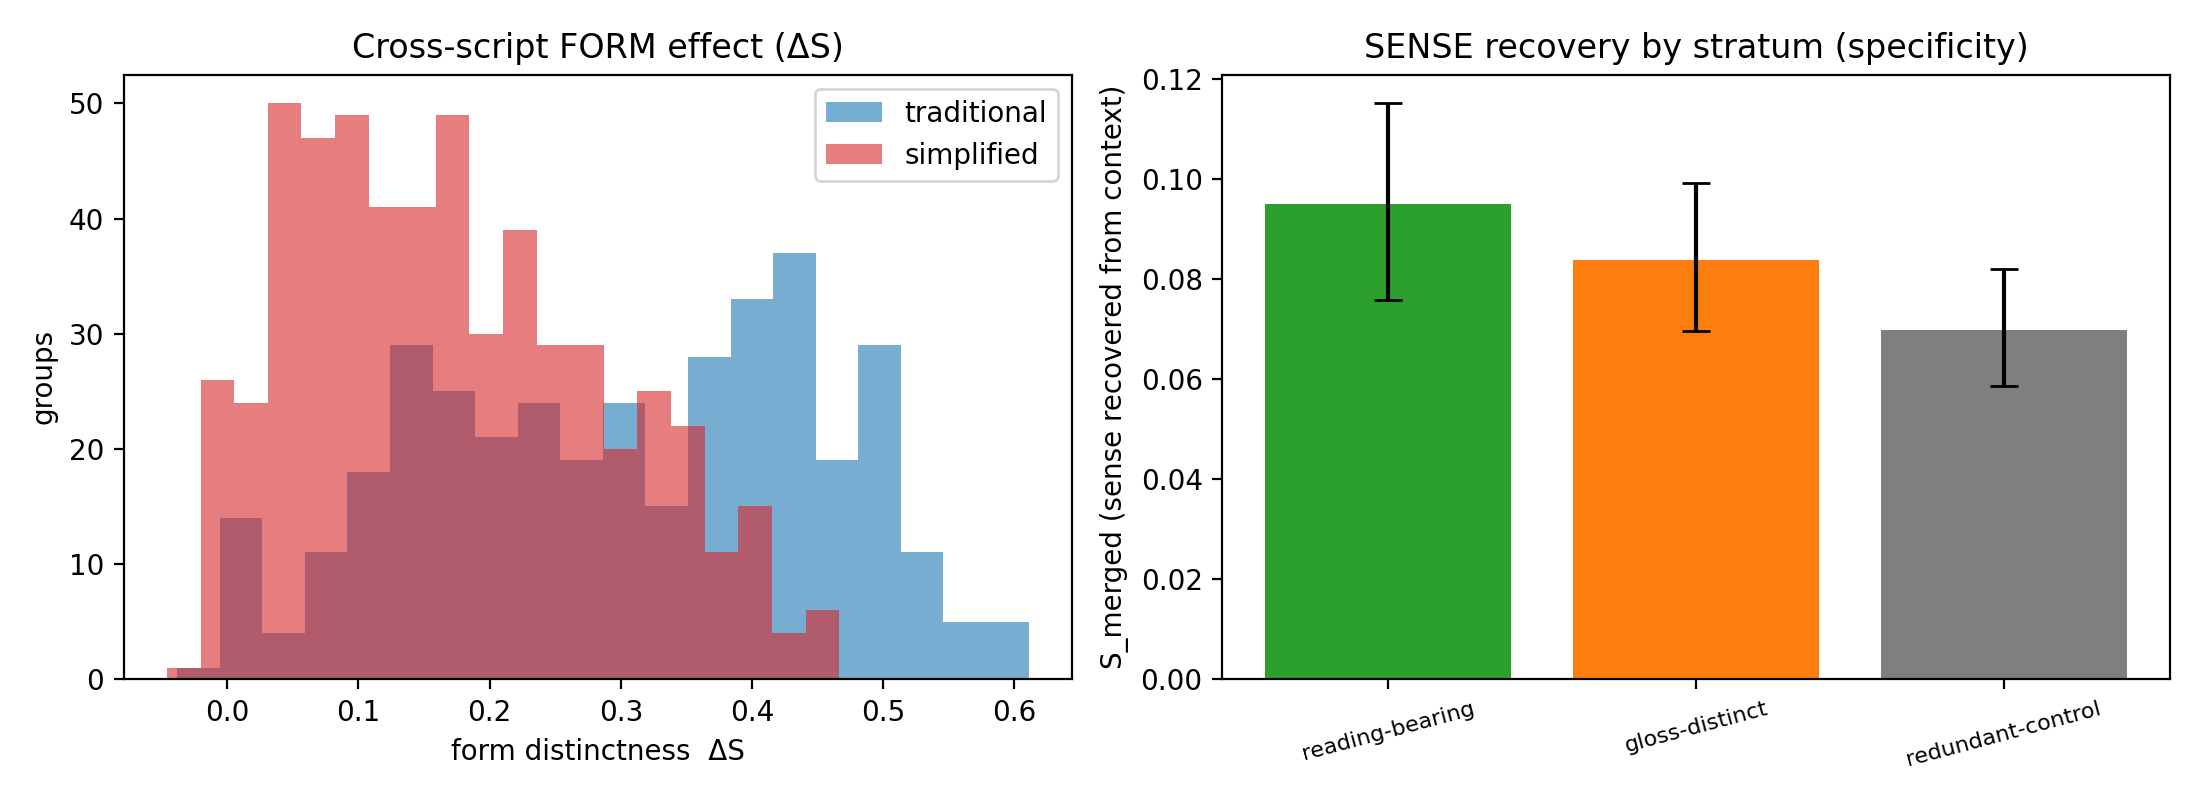
\includegraphics[width=\columnwidth]{fig_results.png}
\caption{Left: cross-script form distinctness $\Delta S$ by script orientation.
Right: sense recovery $S_{\mathrm{merged}}$ by stratum, with 95\% bootstrap CIs.
The form effect separates the scripts; the sense effect separates genuine
distinctions from redundant controls.}
\label{fig:results}
\end{figure}

\section{Discussion}
The 1955 table was issued as housekeeping: a removal of redundant duplicates. Our
census says that judgement was right about three quarters of the time and wrong
for a measurable quarter, where the abolished form carried a reading or a name
that the orthodox form does not. Language models, which see only the surviving
form in context, behave in a way that lines up with this structure: they recover
from context precisely the distinctions that were genuine, and not the redundant
ones, and they do so whether trained on Traditional or Simplified text. What
Traditional training adds is not better meaning recovery but a sharper
representation of the abolished \emph{forms} themselves, visible only because the
token vocabulary is held identical across the panel. The distinction lives in the
weights, and it lives there because the Traditional text that Taiwan's tradition
preserves still uses the forms on the page.

\noindent\textbf{Where the distinctions survive.} The abolished forms remain a
living standard only in the Traditional-script tradition, which is also where the
Traditional-trained models that encode them most strongly originate. The
phenomenon is therefore observable only across the strait: the mainland standard
is itself the instrument that removed the forms.

\section{Limitations}
The sense-recovery effect is small in absolute terms (silhouettes near 0.07 to
0.10) and significant rather than large; we lean on the calibrated null and the
redundant control rather than on magnitude. The gloss-based typology is a proxy,
corroborated by the radical at 74.5 percent but not by a native-speaker gold
standard. Many abolished variants are rare and fall outside the model vocabulary;
we address this by restricting the form analysis to real tokens and the sense
analysis to real orthodox forms, but a vocabulary covering the full variant
inventory would allow a cleaner form comparison. The probe corpora are classical
and encyclopaedic registers, whose sense frequencies are not those of general
language, so we report the information-theoretic result under a uniform prior.

\section{Conclusion}
Script reform in mainland China removed meaning twice: once by merging shapes, and
once by abolishing variants. We reconstructed the complete 1955 variant-abolition
population, quantified what it removed, and found that most of it was redundant
but a measurable quarter was not, with 90.9 percent of the upper-bound distinction
unrecoverable from sound. Probing five shared-vocabulary models, we found that
they recover the genuine erased distinctions from context, specifically and above
a null, while the representation of the abolished forms themselves is sharper in
models trained on Traditional text. The Traditional orthography that Taiwan
preserves is, in a measurable sense, a record of distinctions that the variant
tables removed.

\section*{Reproducibility}
The dataset is built deterministically from the official 1955 table and the
Unicode Han database; the corpus, models, and statistics (bootstrap intervals,
Cliff's delta, permutation tests, label-shuffle nulls, Holm-Bonferroni) run
hands-off on a single free Colab T4 in under two hours. The complete dataset,
the data-construction and analysis code, the model-probe pipeline, and all
derived tables and figures are available at
\texttt{https://github.com/aryan35790jp/cross\_straight\_chinese}.

\begin{thebibliography}{99}
\small
\bibitem{maity2025simplification} A.~Maity. 2025. What Simplification Erased:
Measuring Semantic Mergers from the Cross-Strait Script Divide in Chinese Language
Models. Manuscript.
\bibitem{shannon1948} C.~E.~Shannon. 1948. A Mathematical Theory of
Communication. \emph{Bell System Technical Journal}, 27(3):379--423.
\bibitem{rousseeuw1987} P.~J.~Rousseeuw. 1987. Silhouettes: a graphical aid to
the interpretation and validation of cluster analysis. \emph{J.\ Comput.\ Appl.\
Math.}, 20:53--65.
\bibitem{cliff1993} N.~Cliff. 1993. Dominance statistics: Ordinal analyses to
answer ordinal questions. \emph{Psychological Bulletin}, 114(3):494--509.
\bibitem{holm1979} S.~Holm. 1979. A simple sequentially rejective multiple test
procedure. \emph{Scandinavian Journal of Statistics}, 6(2):65--70.
\bibitem{efron1979} B.~Efron. 1979. Bootstrap methods: another look at the
jackknife. \emph{The Annals of Statistics}, 7(1):1--26.
\bibitem{tenney2019} I.~Tenney, D.~Das, and E.~Pavlick. 2019. BERT Rediscovers the
Classical NLP Pipeline. In \emph{Proc.\ ACL}, 4593--4601.
\bibitem{hewitt2019} J.~Hewitt and C.~D.~Manning. 2019. A Structural Probe for
Finding Syntax in Word Representations. In \emph{Proc.\ NAACL-HLT}, 4129--4138.
\bibitem{cui2021} Y.~Cui, W.~Che, T.~Liu, B.~Qin, and Z.~Yang. 2021. Pre-Training
with Whole Word Masking for Chinese BERT. \emph{IEEE/ACM TASLP}, 29:3504--3514.
\bibitem{ckip} CKIP Lab, Academia Sinica. CKIP Transformers: Traditional Chinese
Transformer Models. \texttt{https://github.com/ckiplab/ckip-transformers}.
\bibitem{unihan} The Unicode Consortium. Unicode Han Database (Unihan), UAX \#38,
Unicode 17.0.0.
\bibitem{opencc} OpenCC contributors. Open Chinese Convert (OpenCC).
\texttt{https://github.com/BYVoid/OpenCC}.
\bibitem{moedict} Ministry of Education, R.O.C. Dictionary of Chinese Character
Variants (異體字字典).
\end{thebibliography}

\end{document}
